\appendix
\part*{\appendixname}

\begin{figure}[!ht]
    \centering
    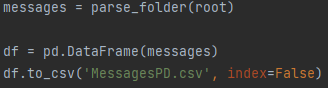
\includegraphics[width=0.75\textwidth]{images/Dataframe_messages.PNG}
    \caption{Python Code - Export in .CSV Datei} 
    \label{fig:dataframeparstetocsv}
\end{figure}

\begin{figure}[!ht]
    \centering
    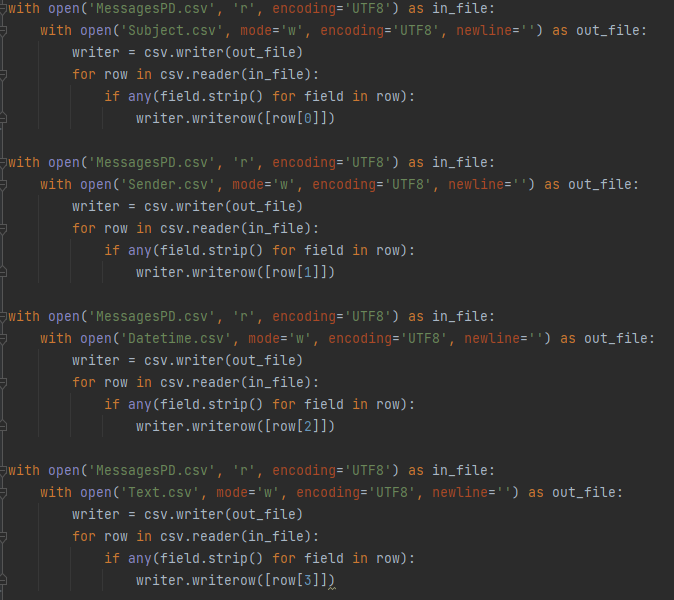
\includegraphics[width=0.75\textwidth]{images/Einzelne_Eigenschaften_in_CSV.PNG}
    \caption{Python Code - Extrahieren der einzelnen Eigenschaften in separate .csv-Dateien} 
    \label{fig:csvseparation}
\end{figure}

\begin{figure}[!ht]
    \centering
    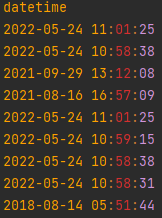
\includegraphics[width=0.50\textwidth]{images/datetime.PNG}
    \caption{E-Mail Eigenschaft datetime} 
    \label{fig:datetime}
\end{figure}

\begin{figure}[!ht]
    \centering
    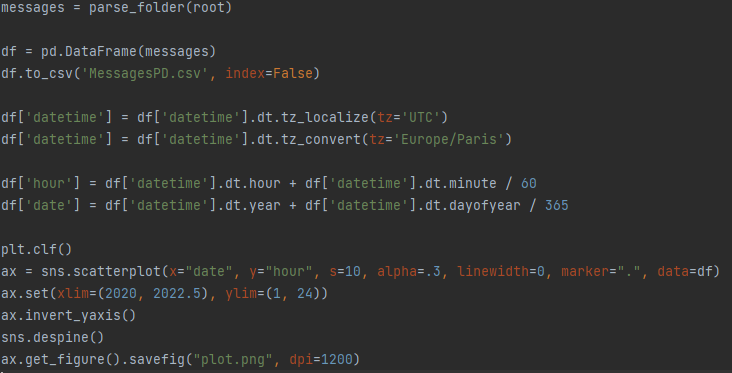
\includegraphics[width=0.75\textwidth]{images/Auswertung_Zeiten.PNG}
    \caption{Python Code - Auswertung hinsichtlich der Empfangszeiten} 
    \label{fig:emailsdatetime}
\end{figure}

\begin{figure}[!ht]
    \centering
    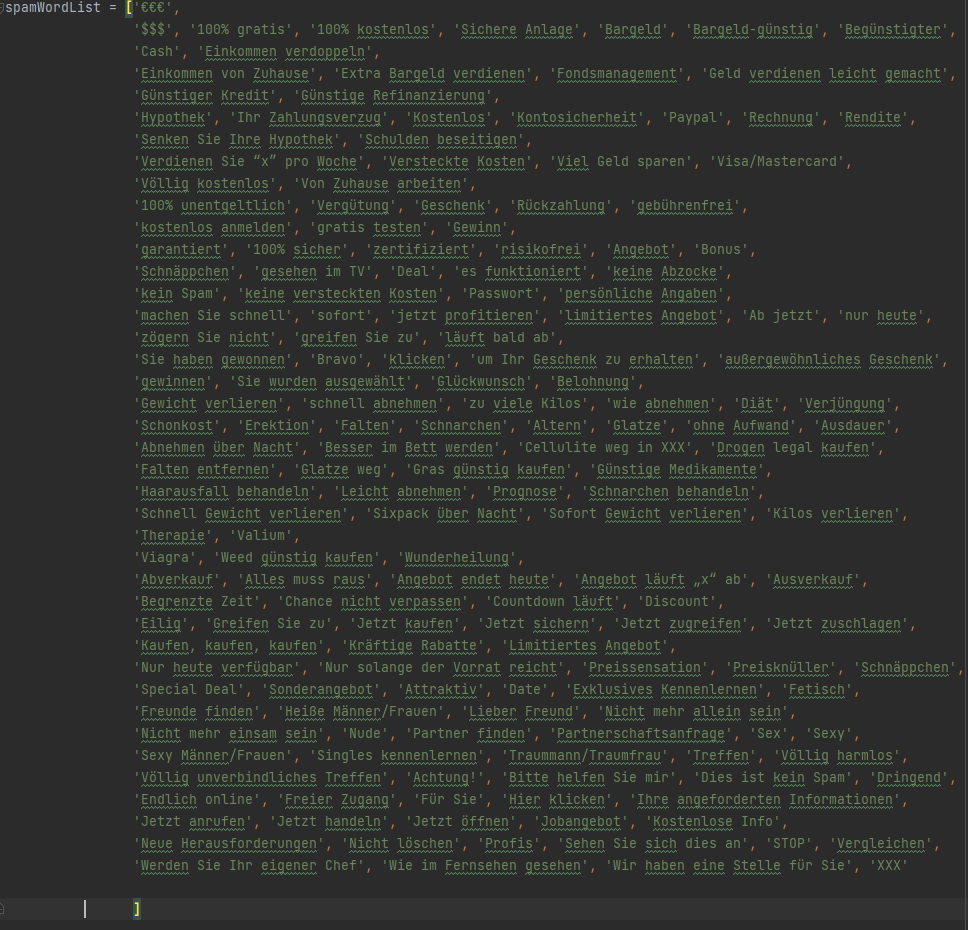
\includegraphics[width=0.75\textwidth]{images/Spamwortliste.PNG}
    \caption{Spamwortliste} 
    \label{fig:spamwortliste}
\end{figure}

\begin{figure}[!ht]
    \centering
    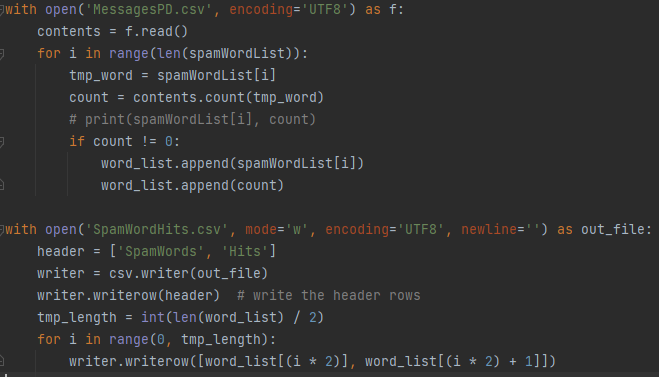
\includegraphics[width=0.75\textwidth]{images/python_Spamwordsearch.PNG}
    \caption{Python Code - Durchsuchen der E-Mails nach Schlagworten} 
    \label{fig:spamwordsearch}
\end{figure}


\newpage
\clearpage